\documentclass{beamer}

 

\usepackage{graphicx}
 
\usepackage{multirow}
\usepackage{array}
\newcolumntype{L}[1]{>{\raggedright\let\newline\\\arraybackslash\hspace{0pt}}m{#1}}

\usetheme[hideothersubsections]{HRTheme}
\usepackage{beamerthemeHRTheme}

\newcommand{\red}[1]{
\textcolor{red}{#1}
}
\usepackage{graphicx}
\usepackage[space]{grffile}
\usepackage{listings}

\lstset{language=C,
basicstyle=\ttfamily\footnotesize,
mathescape=true,
breaklines=true}

\usepackage[utf8]{inputenc}

\title{High performance encapsulation in Casanova 2}

\author{Abbadi Mohamed}

\institute{Ca' Foscari University (Venice, Italy)\\
Tilburg University (Tilburg, Netherlands)}

\date{}

\begin{document}
\maketitle

\SlideSection{Introduction}
\SlideSubSection{Talk topics}
\begin{slide}{
\item Introduction
\item Tools and languages
\item Encapsulation
\item Problem
\item Idea
\item Details
\item Evaluation
\item Conclusions
}\end{slide}


\SlideSubSection{Games in our society}
\begin{twoPicturesTextSlide}
{
\item Games huge
\item[]
\item[]
\begin{itemize}
\item[]
\item[]
\item[]
\end{itemize}
}
{Figures/nomans}
{Figures/halo}
\end{twoPicturesTextSlide}



\SlideSubSection{Games in our society}
\begin{twoPicturesTextSlide}
{
\item Games huge
\item Games are not meant only for entertainment
\item[]
\begin{itemize}
\item Serious games
\item Indie games
\item Research games
\end{itemize}
}
{Figures/hospital}
{Figures/serious_game}
\end{twoPicturesTextSlide}



\SlideSubSection{Costs in game development}
\begin{slide}{
\item Arising from game content, coding, debugging, maintenance, etc.
\item Serious games and research projects do not enjoy the same budgets of the entertainment game industry
\item Costs must stay in-check
}\end{slide}




\SlideSubSection{Games are complex}
\begin{slide}{
\item Complexity arising from the difficulty of expressing game dynamics
\pause
\item How do we reduce such difficulty?
}\end{slide}

\SlideSubSection{Tools and languages}
\begin{slide}{
\item Try to provide support to reduce difficulties in game development
\pause
\item Tools, limited
\item Languages, expressive
\pause
\item Our research focus on languages
}\end{slide}

\SlideSection{A domain programming language}
\SlideSubSection{Casanova 2}
\begin{slide}{
\item A domain specific language
\pause
\item Casanova 2 is:
\begin{itemize}
\item OO, Functional, and Declarative
\item Entities
\item Rules
\begin{itemize}
\item Effect system
\item Only way only to change the game state
\end{itemize}
\end{itemize}
}\end{slide}


\SlideSubSection{Design strategies in Casanova 2}
\begin{slide}{
\item Take specific shapes in Casanova 2
\pause
\item In particular, we have focused on the consequences of encapsulation on code structure and run-time behavior
\pause
\item[]
\item \textbf{Encapsulation}, \textit{helps developers keeping code readable and maintainable, hence help to reduce development costs}
\item[]
\centering
\begin{figure}
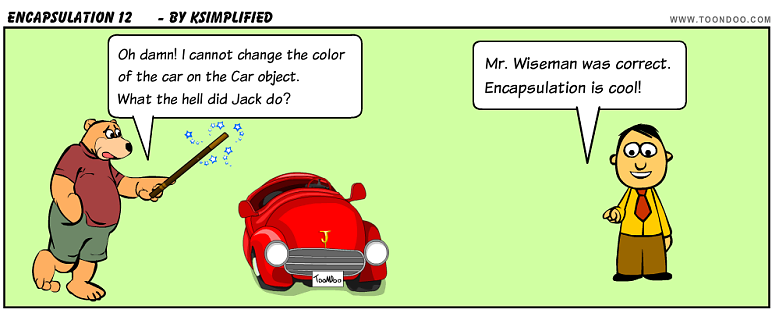
\includegraphics[width = 0.8\textwidth]{Figures/encapsulation-12}
\end{figure}
}\end{slide}


\SlideSection{Problem statement}
\SlideSubSection{First problem statement}
\begin{slide}{
\item To what extent can we take advantage of encapsulation to reduce the difficulty of making games?
}\end{slide}

\SlideSubSection{Encapsulation issues}
\begin{slide}{
\item A a game is run-time applications, hence game code must be performant/fast
\item Performance becomes an issue when dealing with encapsulation
\item Developers avoid encapsulation for highly-coupled and high-performance code
\item[]
\item[]
}\end{slide}

\SlideSubSection{Encapsulation issues: encapsulated code}
\begin{frame}[fragile]{\CurrentSection}
\begin{block}{\CurrentSubSection}
\begin{lstlisting}[frame=box,language=CAML,basicstyle=\tiny,backgroundcolor=\color{white}]
class Route
    Planet Start, Planet End,
    List<Fleet> TravellingFleets,
    Player Owner
    void Update()
      foreach fleet in TravellingFleets
        if End.AttackingFleets.Contains(fleet)
          this.TravellingFleets.Remove(fleet)
class Planet
    List<Fleet> DefendingFleets,
    List<Fleet> AttackingFleets
    void Update()
      foreach route in GetState().Routes
        if route.End = this then
          foreach fleet in route.TravellingFleets
            if distance(fleet.Position, this.Position) < min_dist && fleet.Owner != this.Owner then
              this.AttackingFleets.Add(fleet)
\end{lstlisting}
Nice, it's clear! -:) but ... can't we make it go faster? 
\end{block}
\end{frame}




\SlideSubSection{Encapsulation issues: same semantics but without encapsulation}
\begin{frame}[fragile]{\CurrentSection}
\begin{block}{\CurrentSubSection}
\begin{lstlisting}[frame=box,language=CAML,basicstyle=\tiny,backgroundcolor=\color{white}]
class Route
    Planet Start, Planet End,
    List<Fleet> TravellingFleets
    void Update()
      foreach fleet in this.TravellingFleets
        if distance(fleet.Position, this.Position) < min_dist && fleet.Owner != End.Owner then
            this.TravellingFleets.Remove(fleet)
            End.AttackingFleets.Add(fleet)
\end{lstlisting}
Finally fast -:) but does this code affect readability, so its maintainability?
\end{block}
\end{frame}

\SlideSubSection{Encapsulation issues}
\begin{slide}{
\item A a game is run-time applications, hence game code must be performant/fast
\item Performance becomes an issue when dealing with encapsulation
\item Developers avoid encapsulation for highly-coupled and high-performance code
\item[]
\item PITY!
}\end{slide}

\SlideSubSection{Refined problem statement}
\begin{slide}{
\item \textbf{To what extent can we take advantage of encapsulation in order to produce a high-performance run-time game code?}
\item \textbf{To what extent can we automatize this process?}
}\end{slide}


\SlideSection{Idea}
\SlideSubSection{Optimizing the Planet/Route example}
\begin{slide}{
\item We maintain an index \texttt{FleetIndex} in \texttt{Planet}
\item \texttt{FleetIndex} is the collection of \texttt{Fleet} that satisfy the attacking property
\item A \texttt{Fleet} adds/removes itself from \texttt{FleetIndex} depending on its distance from the \texttt{Planet}
}\end{slide}


\SlideSubSection{Optimization generalization}
\begin{slide}{
\item A predicate $P$, a conditional statement, is based on fields of a type $E_{A}$
\item An index ${I_{A} \in E_{B} \ |\ \forall f \in I_{A}, P(f) = True}$
\item Every entity of type $E_{A}$ got a reference to $E_{B}$. Every entity of type $E_{A}$ is tasked to update its reference inside of $I_{A}$
\item An entity of type $E_{B}$ checks its $I_{A}$ whenever the entity needs to interact with the objects of type $E_{A}$ that satisfy the property $P$
}\end{slide}

\SlideSubSection{Temporal locality of predicates - part I}
\begin{slide}{
\item Predicates belong to entities that exhibit similar behaviors with respect to the time flow
\item We can expect that predicates will exhibit some sort of \textit{temporal locality} on their behaviors
}\end{slide}

\SlideSubSection{Temporal locality of predicates - part II}
\begin{slide}{
\item If we manage to evaluate the predicate only when a field that takes part of the predicate changes then we can achieve a further optimization
\pause
\item We need:
\begin{itemize}
\item a fast wake-up collection where we store predicates and their block of code
\item to active those predicates for some time in order to perform the predicate check whenever a predicate changes its state
\end{itemize}
}\end{slide}





\SlideSection{Details}
\SlideSubSection{Process}
\begin{slide}{
\item[]
\centering
\begin{figure}
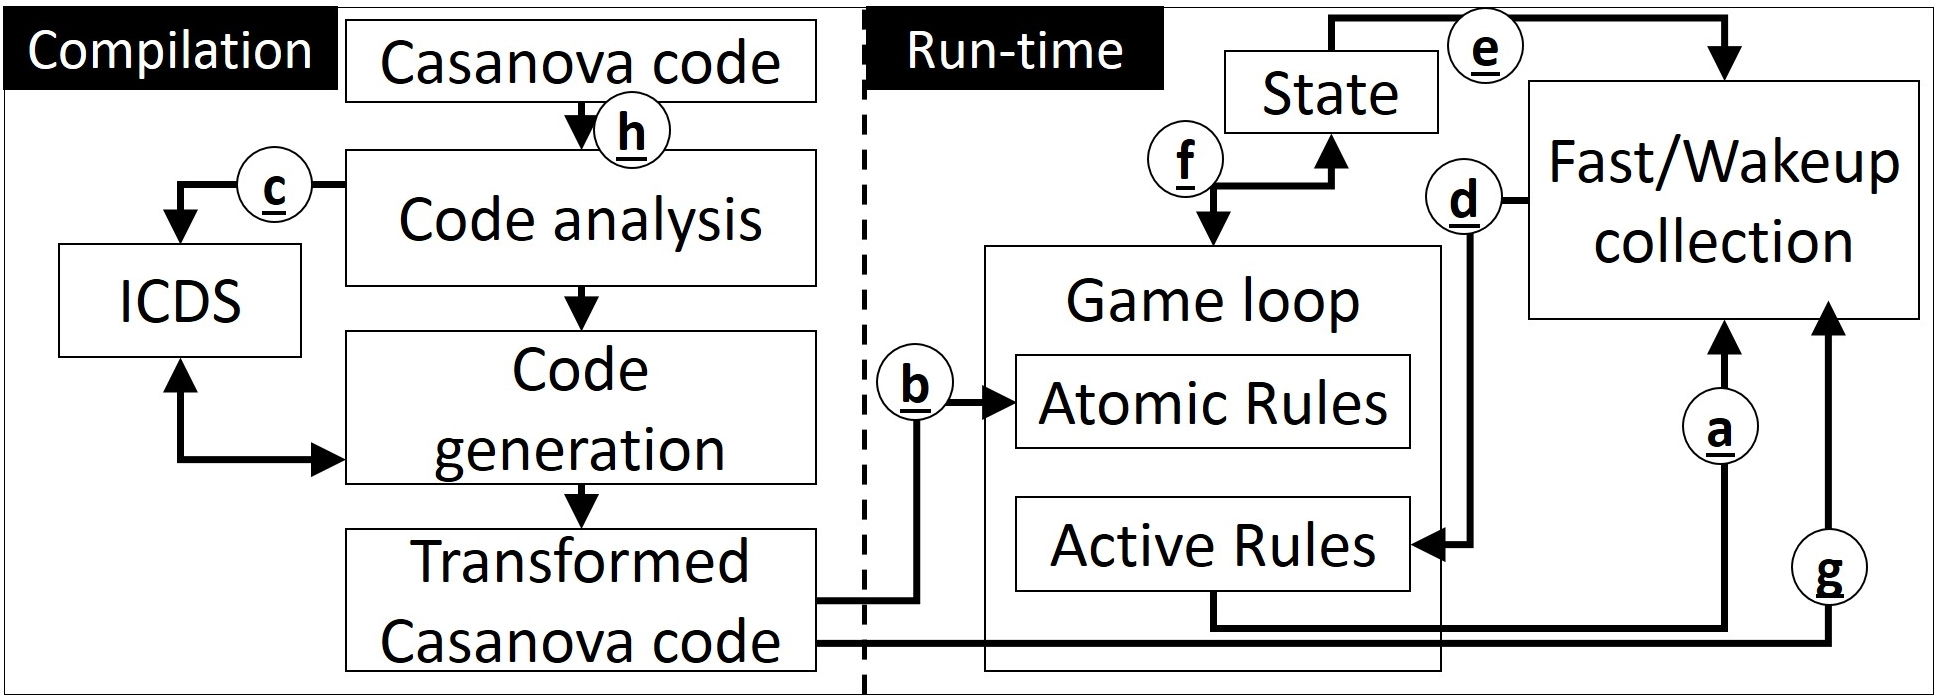
\includegraphics[width = 0.8\textwidth]{Figures/system_description}
\end{figure}
}\end{slide}

\SlideSubSection{Recognizing IC's}
\begin{slide}{
\item[]
\begin{figure}
\centering
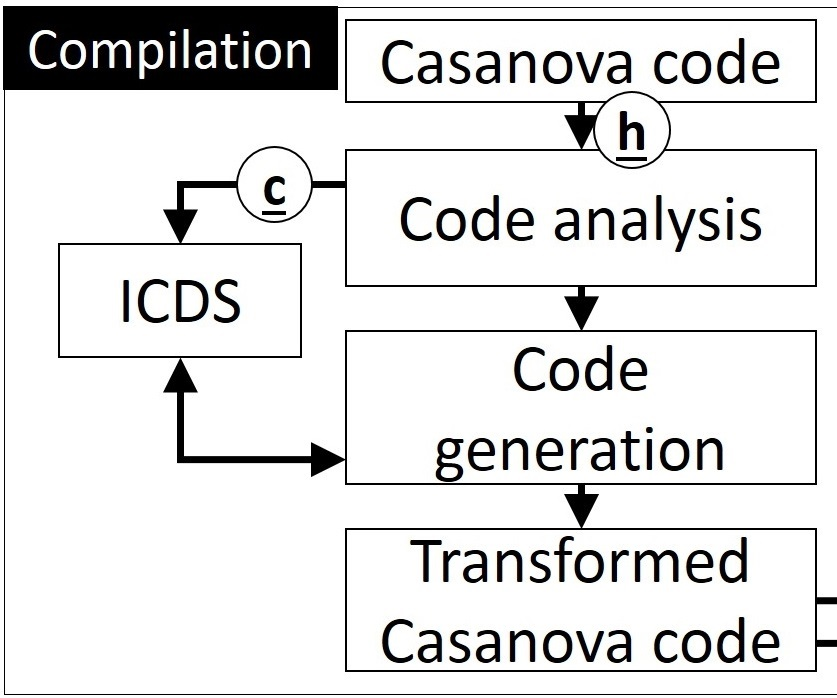
\includegraphics[width = 0.5\textwidth]{Figures/system_description 1}
\end{figure}
\item First we identify the so called interesting conditions (IC) in code
\item Among the all possible IC's we chose only those IC's that are not affected by an atomic rule
}\end{slide}

\SlideSubSection{Run-time efficient sleep/wake-up system}
\begin{pictures2TextSlide}{
\item We store an index that represents the block of code that follows the predicate into a collection
}
{Figures/system_description 2}
{\item We run the block of code (by simply moving its index into the collection of active blocks) whenever the predicate changes to true
\item We keep the block active as long as the evaluation of the predicate yields to true}
\end{pictures2TextSlide}


\SlideSubSection{Some considerations - part I}
\begin{picturetextslide}
{
\item Every instance should take care about its reference inside the fast/wake-up collection
\item In particular it should take into consideration:
\item[]
\begin{itemize}
\item Creation
\item Deletion
\end{itemize}
}
{Figures/system_description 2}
\end{picturetextslide}


\SlideSubSection{Some considerations - part II}
\begin{picturetextslide}
{
\item Dithering is an important property that an entity should exhibit
\item Our system adds a layer of complexity to the run-time system
}
{Figures/system_description 2}
\end{picturetextslide}

\SlideSection{Evaluation}

\SlideSubSection{Code lines comparison}
\begin{frame}[fragile]{\CurrentSection}
\begin{block}{\CurrentSubSection}
\begin{table}
\begin{tabular}{||L{2cm}|L{2cm}|L{2cm}|L{2cm}|L{2cm}}
\hline
\hline
  Original language & Generated language & Optimized code & Lines \\ \hline
  Casanova & - & - & 45 \\
  Casanova & C\# & No & 139 \\
  Casanova & C\# & Yes & 327 \\
  C\# & - & - & 88\\
\hline  
\end{tabular}
\end{table}
\end{block}
\end{frame}


\SlideSubSection{Running time comparison}
\begin{frame}[fragile]{\CurrentSection}
\begin{block}{\CurrentSubSection}
\begin{table}
\begin{tabular}{||L{2cm}|L{2cm}|L{2cm}|L{2cm}|L{2cm}}
\hline
 Platform & Language & Optimized & Performance\\ \hline
\multirow{3}{*}{Monogame}
  & Casanova & No & 0.0159 ms\\
  & Casanova & Yes & 0.0098 ms\\
  & C\# &   - & 0.0147 ms\\ \hline
\multirow{3}{*}{Unity3D}
  & Casanova & No & 0.0257 ms\\
  & Casanova & Yes & 0.0085 ms\\
  & C\# &   - & 0.1642 ms\\ \hline
\hline
\end{tabular}
\end{table}
\end{block}
\end{frame}


\SlideSubSection{Some Casanova games/demos}
\begin{frame}[fragile]{\CurrentSection}
\begin{block}{\CurrentSubSection}
\begin{table}[h!]
  \centering
  \begin{tabular}{ m{2cm} m{2cm} m{2cm} m{2cm} }
  
    \begin{minipage}{.23\textwidth}
      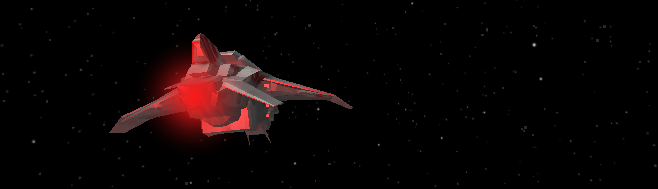
\includegraphics[width=\linewidth]{Figures/a}
    \end{minipage}
    &
        \begin{minipage}{.23\textwidth}
      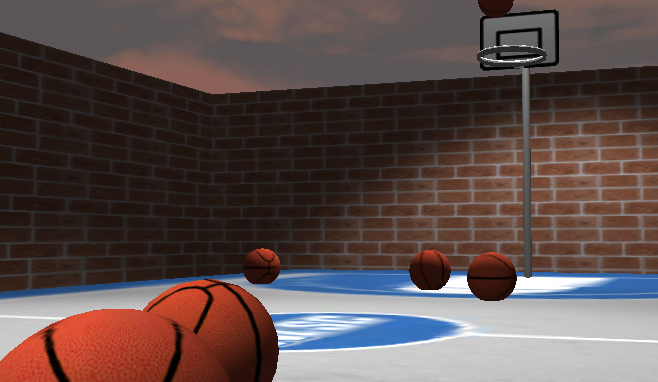
\includegraphics[width=\linewidth]{Figures/b}
    \end{minipage}
    &     
    \begin{minipage}{.23\textwidth}
      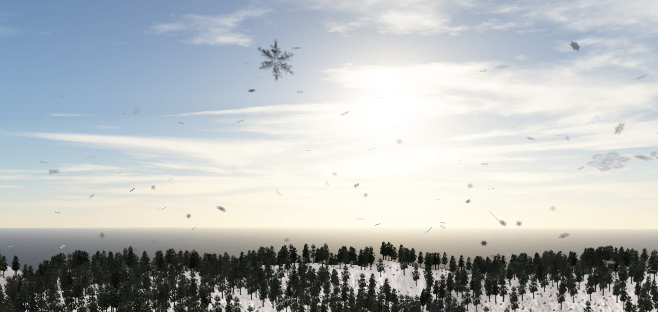
\includegraphics[width=\linewidth]{Figures/c}
    \end{minipage}
    &
    \begin{minipage}{.23\textwidth}
      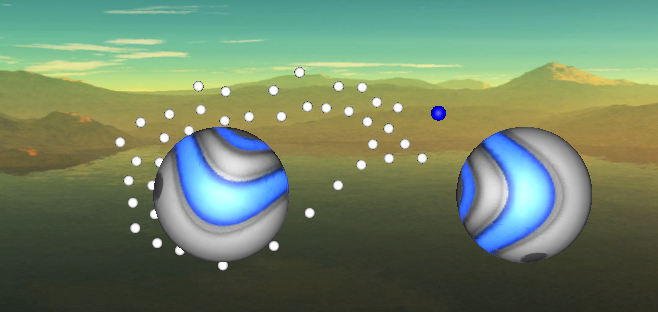
\includegraphics[width=\linewidth]{Figures/d}
    \end{minipage}
    \\ 
        \begin{minipage}{.23\textwidth}
      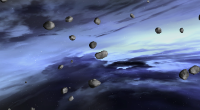
\includegraphics[width=\linewidth]{Figures/e}
    \end{minipage}
    &
        \begin{minipage}{.23\textwidth}
      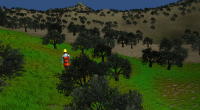
\includegraphics[width=\linewidth]{Figures/f}
    \end{minipage}
    &     
    \begin{minipage}{.23\textwidth}
      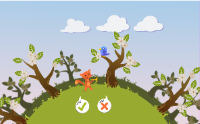
\includegraphics[width=\linewidth]{Figures/g}
    \end{minipage}
    &
    \begin{minipage}{.23\textwidth}
      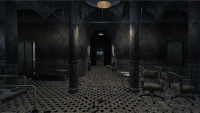
\includegraphics[width=\linewidth]{Figures/h}
    \end{minipage}
    \\ 
    
  \end{tabular}
\end{table}
\centering
\textbf{https://github.com/vs-team/casanova-mk2/wiki}
\end{block}
\end{frame}

\SlideSection{Conclusions \& future works}
\begin{slide}{
\item This work is far to be completed ...
\item We showed that:
\begin{itemize}
\item By using encapsulation, game code may be written in a maintainable way
\item By mean of our solution, encapsulated programs suffer less performance
\item Developers can use safely encapsulation in their design/code, hence costs are reduced
\item Making games for serious games developers and researchers is more accessible
\end{itemize}
}\end{slide}

\begin{frame}{This is it!}
\center
\fontsize{18pt}{7.2}\selectfont
Thank you! :)
\end{frame}

\end{document}

\begin{slide}{
\item ...
}\end{slide}

\begin{frame}[fragile]
\begin{lstlisting}
...
\end{lstlisting}
\end{frame}


